% =====================================================================
%  sections/sec7.tex —— 7 已知例子的六维表示（原文 pp.46–48）
% =====================================================================
\section{已知例子的六维表示}
\label{sec:known}

我们已经说明：$(A_1,A_N)$、$(A_1,D_N)$、$(A_1,E_N)$ 理论都可以用六维 $A_1$ 与 $A_2$ 理论配上适当的非正则奇点来工程化。更一般地，$(A_{k-1},A_{N-1})$ 理论也可以用六维 $A_{k-1}$ 或 $A_{N-1}$ 理论来工程化。下面再给一些例子。

$A_0$、$A_1$、$A_2$、$E_6$、$E_7$、$E_8$ 理论都有六维的秩 $N$ 推广（这些名字来自味对称性，以及 Kodaira 对奇异纤维的分类）。秩 $N$ 的 $E_6$、$E_7$、$E_8$ 理论，可以通过把六维 $A_{3N-1}$、$A_{4N-1}$、$A_{6N-1}$ 理论紧致化在只带正则奇点的三孔球上实现 \cite{46}。

现在我们用非正则奇点来工程化秩 $N$ 的 $A_0$、$A_1$、$A_2$ 理论。把 $A_{2N-1}$ 理论紧致化在带下述非正则奇点的球上：
\begin{equation}
A_0:\quad \Phi = \frac{1}{z^{4-1/2}}\diag(\underbrace{1,1,\dots 1}_{N},\ \underbrace{-1,-1,\dots -1}_{N}) + \cdots
\label{eq:7.1}\tag{7.1}
\end{equation}
其领头阶系数有 $N$ 个根 $1$ 与 $N$ 个根 $-1$，次领头阶的项具有同样的模式。这些算子的维数为 $\tfrac{6}{5},\ 2\times\tfrac{6}{5},\ \dots,\ \tfrac{6}{5}N$。

秩 $N$ 的 $A_1$ 理论用 $A_{2N-1}$ 理论与下述非正则奇点来工程化：
\begin{equation}
A_1:\quad \Phi = \frac{1}{z^4}\diag(\underbrace{1,1,\dots 1}_{N},\ \underbrace{-1,-1,\dots -1}_{N}) + \cdots
\label{eq:7.2}\tag{7.2}
\end{equation}
其中 $\tfrac{1}{z^3}\dots\tfrac{1}{z}$ 的系数与领头阶具有同类型的矩阵。谱的标度维数为 $\tfrac{4}{3},\ \tfrac{8}{3},\ \dots,\ \tfrac{4}{3}N$，并且有一个质量参数。

秩 $N$ 的 $A_2$ 理论需要两个奇点：其一为非正则奇点，形式为
\begin{equation}
A_2:\quad \Phi = \frac{1}{z^3}\diag(\underbrace{1,1,\dots 1}_{N},\ \underbrace{-1,-1,\dots -1}_{N}) + \cdots
\label{eq:7.3}\tag{7.3}
\end{equation}
其中 $\tfrac{1}{z^2}\dots\tfrac{1}{z}$ 的系数与领头阶具有同类型的矩阵；其二是一个杨图为 $[N,N]$ 的正则奇点。该理论有 $N$ 个库仑分支算子，维数为 $\tfrac{3}{2},\ \tfrac{3}{2}\times 2,\ \dots,\ \tfrac{3}{2}\times N$，还有两个质量参数。

秩 $N$ 的 $A_1$ 与 $A_2$ 理论的镜像理论画在图 \ref{fig:20} 中。利用谱的信息与镜像对称，可以算出中心荷 $a$ 与 $c$。对秩 $N$ 的 $A_1$ 理论，镜像的库仑分支维数为 $2N-1$，于是
\begin{equation}
2a-c = \frac{1}{4}\sum_i\bigl(2D(u_i)-1\bigr) = \frac{1}{12}(N+4N^2),\qquad
a-c = -\frac{2N-1}{24},
\label{eq:7.4}\tag{7.4}
\end{equation}
从而
\begin{equation}
a = \frac{1}{24}(-1+4N+8N^2),\qquad c = \frac{1}{12}(-1+3N+4N^2).
\label{eq:7.5}\tag{7.5}
\end{equation}
类似地，对秩 $N$ 的 $A_2$ 理论，镜像的库仑分支维数为 $3N-1$，于是
\begin{equation}
2a-c = \frac{1}{8}(N+3N^2),\qquad a-c = -\frac{3N-1}{24},
\label{eq:7.6}\tag{7.6}
\end{equation}
从而
\begin{equation}
a = \frac{1}{24}(-1+6N+9N^2),\qquad c = \frac{1}{24}(-2+9N+9N^2).
\label{eq:7.7}\tag{7.7}
\end{equation}
这些结果与 \cite{21} 一致。

文献 \cite{47,48} 用奇点理论找到的一些 SCFT，同样可以用非正则奇点来工程化。只举一个例子：所谓的 W13 理论，它在奇点处的 Seiberg--Witten 曲线为
\begin{equation}
x^4 + x y^4 = 0 .
\label{eq:7.8}\tag{7.8}
\end{equation}
显然，这就是用六维 $A_3$ 理论构造的 type II SCFT。

\begin{figure}[tbp]
\centering
% Figure 20 -- (a) 3d mirror for rank N A_1 theory, (b) for rank N A_2 theory
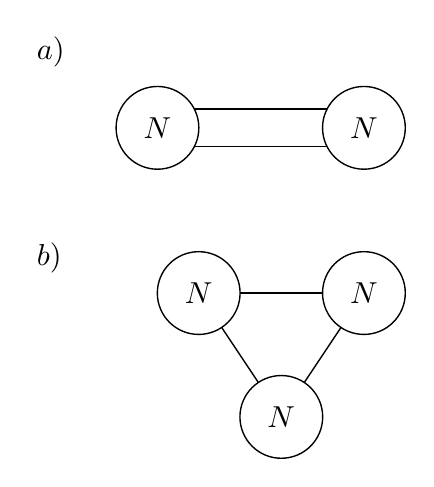
\begin{tikzpicture}[x=1pt,y=1pt,>=stealth,line width=0.5pt,
   nd/.style={circle,draw,fill=white,minimum size=29.9pt,inner sep=0pt,
              font=\fontsize{11}{11}\selectfont}]
  % ---------------- a) ----------------
  \draw (59.15,140.1) -- (133.75,140.1);
  \draw (59.15,126.6) -- (133.75,126.6);
  \node[nd] at (59.15,133.35) {$N$};
  \node[nd] at (133.75,133.35) {$N$};
  \node[anchor=base west,font=\fontsize{10.7}{10.7}\selectfont] at (12,158) {$a)$};
  % ---------------- b) ----------------
  \draw (74.05,73.65) -- (133.75,73.65);
  \draw (74.05,73.65) -- (103.9,28.9);
  \draw (133.75,73.65) -- (103.9,28.9);
  \node[nd] at (74.05,73.65) {$N$};
  \node[nd] at (133.75,73.65) {$N$};
  \node[nd] at (103.9,28.9) {$N$};
  \node[anchor=base west,font=\fontsize{10.7}{10.7}\selectfont] at (12,83.5) {$b)$};
\end{tikzpicture}

\caption{(a) 秩 $N$ 的 $A_1$ 理论的三维镜像。(b) 秩 $N$ 的 $A_2$ 理论的三维镜像。}
\label{fig:20}
\end{figure}
